\documentclass[12pt]{exam}
\setlength{\oddsidemargin}{0in}
\setlength{\evensidemargin}{0in}
\setlength{\textwidth}{6.8in}
\setlength{\parindent}{0in}
\setlength{\parskip}{\baselineskip}

\usepackage{graphicx} % Required for inserting images
\usepackage{amsmath,amsfonts,amssymb}
\usepackage{xcolor}
\usepackage{hyperref}
\usepackage{ dsfont }
\usepackage{tikz}
\title{CSCI-246 Discrete Structures HW 10}
\author{Instructor: Adiesha Liyanage}
\date{November 05 2024}

\begin{document}

\maketitle

\hrulefill
\\
\\
\textbf{Objective}
\begin{itemize}
    \item Understanding graph definitions.
    \item Understanding the problem solving process.
    \item Understanding how to solve a problem using graph based approach.
\end{itemize}

\textbf{Submission requirements}
\begin{itemize}
    \item \textbf{\textit{Type or clearly hand-write}} your solutions into a \textbf{\textit{PDF FORMAT.}} 
    \item \textbf{\textit{DO NOT UPLOAD images.}}
    \item \textbf{\textit{non-pdf or emailed solutions will not be graded.}}
    \item \textbf{If you take pictures of your handwritten homework, put it into pdf format.}
    \item \textbf{\textit{Start each problem on a new page.}}
    \item Follow the model that you have learned during the lectures for proofs.
    \item Do not wait until the last minute to submit the assignment.
    \item You can submit any number of times before the deadline. 
    \item If you are using latex, and you do not know how to type a symbol, use the following website. You can draw the symbol here and it will give you the latex code and the packages that you have to import. \url{https://detexify.kirelabs.org/classify.html}
    \item If you are using latex to write the answer, you can use overleaf to make your life easier. \textbf{Overleaf is a free, online platform that helps users create and publish scientific and technical documents using LaTeX, a markup-based document preparation system}
    \item If you do not understand a problem, ask questions during/after the lectures, or during office hours or via discord.
    \item Go to TA office hours and talk with them and ask for help.
    \item \textbf{\textit{Do not use generative AI to write answers.}} 
\end{itemize}

Homework 02 contains \textbf{3 questions}.

\section{Q1}
In the lecture on special graphs, we proved that if a graph contains a triangle, then it is not bipartite.
\begin{enumerate}
    \item What is the converse of this statement?
    \item What is the inverse of this statement?
    \item Is the converse of the statement true or false?
    \item Prove your answer to the previous question.
\end{enumerate}

\section{Q2} 
In the lectures, we learned that distance between two nodes is the length of the shortest path between them. The \textbf{Diameter} of a graph is the largest distance between any two nodes in the graph. For example, for the following graph, the diameter is $3$, which is the distance between $A$ and $E$. One of the shortest paths between $A$ and $E$ is $(A, B, D, E)$.

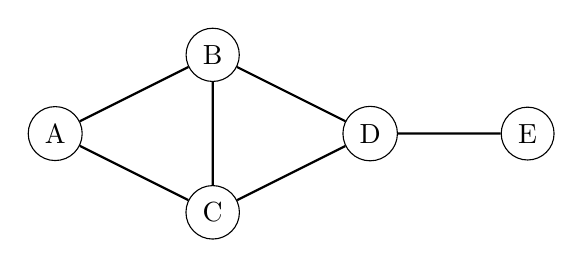
\begin{tikzpicture}[scale=1,auto,node distance=2cm]
    % Nodes
    \node[circle, draw] (A) at (0,0) {A};
    \node[circle, draw] (B) at (2,1) {B};
    \node[circle, draw] (C) at (2,-1) {C};
    \node[circle, draw] (D) at (4,0) {D};
    \node[circle, draw] (E) at (6,0) {E};
    
    % Edges
    \path[draw,thick]
        (A) -- (B)
        (A) -- (C)
        (B) -- (C)
        (B) -- (D)
        (C) -- (D)
        (D) -- (E);
\end{tikzpicture}

\begin{enumerate}
    \item What could be the largest diameter of a connected graph with $n$ nodes can have and \textbf{explain your answer.}
    \item What could be the smallest diameter that a connected graph with $n$ nodes can have and explain the answer?
    \item Draw the above two graphs for $n = 5$.
\end{enumerate}



\section{Q3}
\begin{enumerate}
    \item Suppose that Alice has exactly $160$ friends, and each of her friends has exactly $160$ friends---that is, a friend of Alice knows Alice and $159$ \textbf{other} people. (Note that Alice’s friends’ sets of friends can overlap.) Let $S$ denote the set of people that Alice knows directly or with whom Alice has a mutual friend. What’s the largest possible value of $|S|?$. \textbf{Explain how you got this answer using graph based approach.}
    
    \textbf{Hint: Think of these friendships in terms of a graph. You can create a node for each person and connect them with an undirected edge if they are friends. How can you create a graph such that the set $S$ is maximized---If you answer this question then you can come up with an answer to this question?}
    \item For the set $S$ defined above, what’s the smallest possible value of $|S|$? Explain what type of graph would that be if people are defined as nodes and friendships are defined as an undirected edge.
    \item Let $u$ be a node in an undirected graph $G$. Prove that $u’s$ degree is at most the sum of the degrees of $u’s$ neighbors. Hint: use direct proof.
\end{enumerate}
\end{document}
